\documentclass[12pt]{examdesign}
\XeTeXlinebreaklocale "zh"
\XeTeXlinebreakskip=0pt plus 1pt minus 0.1pt
\usepackage{fontspec}
\usepackage{xeCJK}
\usepackage[b4paper,margin=0.75in,bottom=1in]{geometry}
\setCJKmainfont{Noto Serif CJK TC}
\usepackage{booktabs}
\usepackage{graphicx}
\usepackage{siunitx} 
\usepackage[siunitx]{circuitikz} 
\usepackage{tikz}
%\usepackage{lastpage}
%\usepackage{fancyhdr}
%\pagestyle{fancy}
\headheight=15pt


\graphicspath{{../images/}}

\renewcommand{\baselinestretch}{1.3}
\renewcommand{\figurename}{圖}
\newcommand{\SchoolName}{Taipei Municipal Heping High School}
\newcommand{\zhSchoolName}{臺北市立和平高級中學}
\newcommand{\subjectexamtop}{104 學年度高三物理平時考試卷}
\newcommand{\subjectkeytop}{104 學年度高三物理平時考答案卷}
\newcommand{\subjectendmattertop}{104 學年度高三物理平時考答題卷}

\newcommand{\Scope}{Chapter 7 電流}
\newcommand{\DateTime}{\today}
\everymath{\displaystyle}

%\renewcommand{\headrulewidth}{0pt}
%\cfoot{\thepage}}
%\cfoot{\thepage /\pageref{LastPage}}
%\footskip = 1cm


%\fancyhf{}

%\rfoot{Page \thepage \hspace{1pt} of \pageref{LastPage}}




\begin{examtop}
\begin{center}
{\Large \zhSchoolName}\\[3mm]
{\LARGE \subjectexamtop}\\
Quiz 1 \quad 範圍: \Scope  \hfill Date: \DateTime
\hrule
\end{center}
\end{examtop}

\begin{keytop}
\begin{center}
{\Large \zhSchoolName}\\[3mm]
{\LARGE \subjectkeytop}\\
Quiz 1 \quad 範圍: \Scope  \hfill Date: \DateTime
\hrule
\end{center}
\end{keytop}

\ShortKey
\NoRearrange

\begin{document}

\begin{shortanswer}[
suppressprefix,examcolumns=2,keycolumns=2]

\begin{question}
通過導線的電流為 40 \si{\mA}
求 1 分鐘內通過導線截面的電子數目有多少?
($ 1 e = 1.6 \times 10^{-19} $ C)
\begin{answer}
$ 1.5 \times 10^{19}$
\end{answer}
\end{question}

\begin{question}
有一理想電池連接一燈泡﹐
流經燈泡的電流為 100 \si{\mA},
若電池的電動勢為 1.5 \si{\volt}﹐
求在 1 小時內電池消耗多少化學能?
\begin{answer}
540 \si{\joule}
\end{answer}
\end{question}

\begin{question}
某電解槽中﹐
有帶電量為 $+e$﹑
$-2e$ 的正﹑負離子 ($1e = 1.6 \times 10^{-19}$ C)﹐
接通電池後﹐
測得電流為$ 2.0 \times 10^{-6} $ \si{\ampere}﹐
方向向右。
倘若在 $1.0 \times 10^{-2}$ 秒內﹐
向右通過某截面的正離子數為 $4.0 \times 10^{10}$ 個﹐
則流過此截面的負離子數為多少個?
%\begin{center}
%\includegraphics[width=.2\textwidth]{ex7-10.png}
%\end{center}
\begin{answer}
$ 4.25 \times 10^{10}$
\end{answer}
\end{question}

\begin{question}
一電動勢為 12 \si{\volt}﹑內電阻為 0.05 \si{\ohm} 的汽車電池﹐
以 20 \si{\ampere} 的電流充電﹐
求:\\
(1) 電池兩端的電位差為多少?\\
(2) 須提供充電中的電池之電功率為多少?
\begin{center}
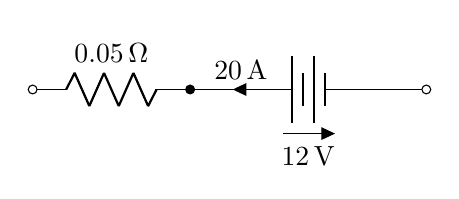
\begin{tikzpicture}
%\ctikzset{bipoles/thickness=2}
%\tikzstyle{every node}=[font=\small]
%\draw [red!40](0,-2) grid (5,2);
\draw (0,0) to[R,l=0.05<\ohm>,o-*] (2,0)
     to[battery,v_=12<\volt>,-o,i<=20<\ampere>] (5,0) ;
\end{tikzpicture}
\end{center}
\begin{answer}
(1) 13 \si{\volt}; (2) 260 \si{\watt}
\end{answer}
\end{question}

\begin{question}
有一個電湯匙的電阻為 60 \si{\ohm}﹐
連接在 100 \si{\volt} 的電壓下﹐
求︰\\
(1) 此電湯匙工作 1 小時產生的熱有多少?\\
(2) 若將此電湯匙浸泡在裝有質量為 500 g 的水之容器中﹐
假設 42\% 的熱被水吸收﹐
則 10 分鐘後﹐水溫升高多少?
\begin{answer}
(1) $6 \times 10^5$ J; (2) $20^\circ$C
\end{answer}
\end{question}

\begin{question}
a,b 間的端電壓為 4.0 V﹑
$\otimes$ 為燈泡﹐
M 為馬達﹐
馬達端電壓為 6.0 V﹐
求﹕\\
(1) 12 V 電池輸出的電功率為多少?\\
(2) 電池 $\varepsilon$ 的電動勢為何?
%\begin{center}
%\includegraphics[width=.3\textwidth]{ex7-18.png}
%\end{center}
\begin{center}
\begin{circuitikz}
\ctikzset{bipoles/thickness=2}
\tikzstyle{every node}=[font=\small]
%\draw [red!40](0,0) grid (5,4);
\draw (4,3) to[battery,l=12<\volt>,i=I] (0,3) ;
\draw (4,3) to[lamp,l_=4<\ohm>] (4,0) to[R,l=2<\ohm>]
     (2,0) to[battery,l=$\varepsilon$] (0,0) to (0,3);
\fill (0,0) circle (2pt) node[below]{a};
\fill (4,0) circle (2pt) node[below]{b};
\node at (0,1.5)[fill=gray!50,draw,minimum height=5mm,minimum width=1cm] {M}; 
\end{circuitikz}
\end{center}
\begin{answer}
(1) 6.0 \si{\watt}; (2) 3 \si{\volt}
\end{answer}
\end{question}


\begin{question}
以固定電流通過一長度為 $\ell$ 的均勻導線,
其二端電位差是 $\varepsilon_1$,
若將該導線均勻拉長成 $4\ell$ 的長度,
其二端的電位差為 $\varepsilon_2$,
則 $\varepsilon_2$ 是 $\varepsilon_1$ 的幾倍?
\begin{answer}
16
\end{answer}
\end{question}


\begin{question}
將一電阻為 $R$ 的均勻導線繞成圓形線圈。
\begin{center}
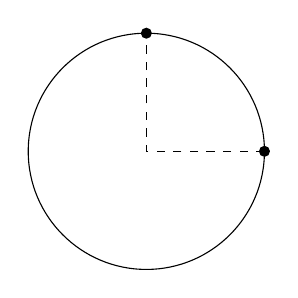
\begin{tikzpicture}
\def\r{1.5}
\draw (0,0) circle (\r);
\fill (0:\r) circle (2pt);
\fill (90:\r) circle (2pt);
\draw [dashed](0:\r)--(0,0)--(90:\r);
\end{tikzpicture}
\end{center}
圓形線圈相隔四分之一圓弧的兩點間電阻值為何?
\begin{answer}
$ \frac{3R}{16} $ 
\end{answer}
\end{question}


\begin{question}
電池的電動勢為 $\varepsilon =6$ V,
無內電阻,
則:\\
(1) 整個電路的等效電阻為多少? \\
(2) 電池供給的電功率為何?
\begin{center}
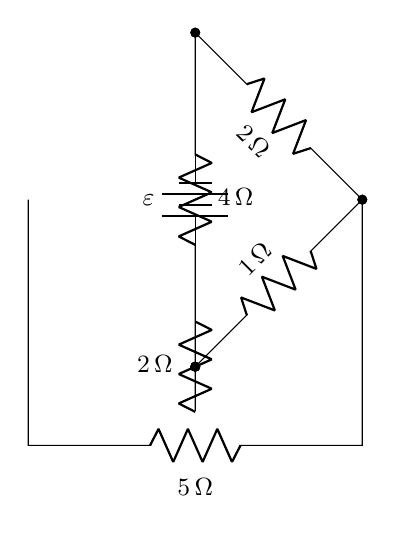
\begin{tikzpicture}
\ctikzset{bipoles/thickness=2}
\tikzstyle{every node}=[font=\small]

\draw (0,0)[R,l=1<\ohm>,*-*] to (45:3) [R,l=2<\ohm>] to +(135:3) [R,l=4<\ohm>]to + (225:3)[R,l=2<\ohm>] to (0,0);
\draw (0,0) [battery,l=$\varepsilon$]to (0,3*1.414);

\draw (45:3) to (45:3 |- 0,-1) to[R,l=5<\ohm>] (225:3 |- 0,-1) to (135:3);
\end{tikzpicture}
\end{center}
\begin{answer}
(1) 2 $\Omega$; (2) 18 W
\end{answer}
\end{question}


\begin{question}
發電廠所發出的電能,
一般須經由長途的輸送線路,
送到各地區的用戶,
因此輸送線路是用電阻很小的銅線製成,
以減少電能的損失。
若發電廠所發出的電功率保持一定,
且輸送線路符合歐姆定律,
當發出電壓變為原來的 10 倍時,
則輸送線路上電能損失的功率變為原來損失的多少倍?
\begin{answer}
0.01
\end{answer}
\end{question}

\begin{question}
電路中六個電阻器之電阻均相同,
A、B 間之電阻器所消耗之電功率為 1 W,
則六個電阻器所消耗之總電功率為何?
\begin{center}
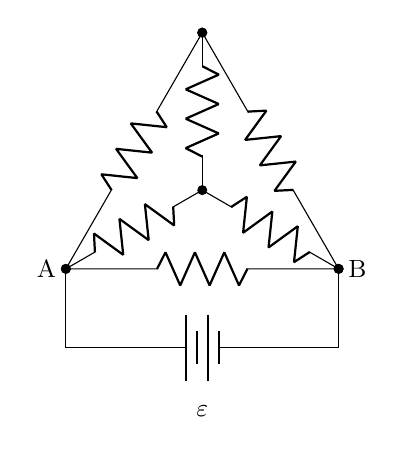
\begin{tikzpicture}
\ctikzset{bipoles/thickness=2}
\tikzstyle{every node}=[font=\small]
%\draw [red!40](-3,-3) grid (3,3);

\coordinate (C) at (90:2) ;
\coordinate (B) at (-30:2);
\coordinate (A) at (210:2);
\draw (0,0) [R,*-] to (A);
\draw (0,0) [R] to (B);
\draw (0,0) [R] to (C);
\draw (A) [R,*-*] to (B) to (C) to (A);
\node at (A) [left] {A};
\node at (B) [right]{B};
\draw (A) to (A |- 0,-2) [battery,l_=$\varepsilon$] to (B |- 0,-2) -- (B);
\end{tikzpicture}
\end{center}
\begin{answer}
2 W
\end{answer}
\end{question}

\begin{question}
有一電鍋規格為110 V、1100 W,
煮一次飯約需 20 分鐘,
則:\\
(1) 煮飯時,流經電鍋的電流為何? \\
(2) 每煮一次飯,約需幾度電能?
\begin{answer}
(1) 10 A; (2) 0.37 度電 
\end{answer}
\end{question}

\begin{question}
求圖中 A  和 B 兩點之間的等效電阻?
\begin{center}
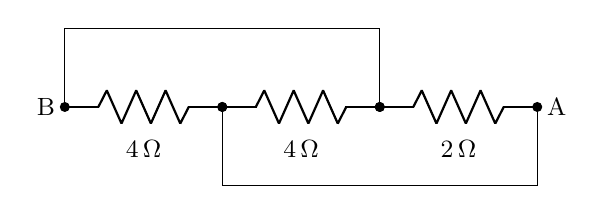
\begin{tikzpicture}
\ctikzset{bipoles/thickness=2}
\tikzstyle{every node}=[font=\small]
\coordinate (A) at (4,0) ;
\coordinate (B) at (2,0);
\coordinate (C) at (0,0);
\coordinate (D) at (-2,0);
\draw (A) [R,l=2<\ohm>,*-*]to (B)[R,l=4<\ohm>] to (C) to (D);
\draw (D)node[left]{B} -- ++(0,1) --++(4,0)--(B);
\draw (C) -- ++ (0,-1) --++(4,0)--(A) node[right]{A};
\end{tikzpicture}
\end{center}
\begin{answer}
1 $\Omega$
\end{answer}
\end{question}


\begin{question}
求圖中 A  和 B 兩點之間的等效電阻?
\begin{center}
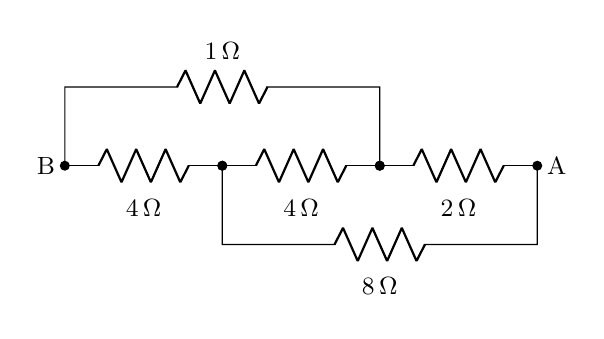
\begin{tikzpicture}
\ctikzset{bipoles/thickness=2}
\tikzstyle{every node}=[font=\small]
\coordinate (A) at (4,0) ;
\coordinate (B) at (2,0);
\coordinate (C) at (0,0);
\coordinate (D) at (-2,0);
\draw (A) [R,l=2<\ohm>,*-*] to (B)[R,l=4<\ohm>] to (C) to (D);
\draw (D)node[left]{B} -- ++(0,1)  to [R,l=1<\ohm>] ++(4,0)--(B);
\draw (C) -- ++ (0,-1) to[R,l_=8<\ohm>] ++(4,0)--(A) node[right]{A};
\end{tikzpicture}
\end{center}
\begin{answer}
2.4 $\Omega$
\end{answer}
\end{question}


\begin{question}
均勻電阻線等切成 $n$ 等份,
全部串聯起來與全部並聯起來的等效電阻之比值為何?
\begin{answer}
$ n^2 $
\end{answer}
\end{question}



\end{shortanswer}



\begin{examclosing}
\vfill
\begin{center}
{\Large \SchoolName}\\[3mm]
\bigskip
班級:\underline{\qquad \qquad} \qquad
座號:\underline{\qquad \qquad} \qquad
姓名:\underline{\qquad \qquad \qquad \qquad\qquad} \qquad
\end{center}
\bigskip

%You are on page \thepage\ of \pageref{LastPage}

\begin{center}
\begin{tabular}{|p{3.5cm}|p{3.5cm}|p{3.5cm}|p{3.5cm}|p{3.5cm}|}
\toprule
1&2&3&4(1)&4(2)\\
\midrule
&&&&\\
&&&&\\
&&&&\\
\midrule
5(1)&5(2)&6(1)&6(2)&7(1)\\
\midrule
&&&&\\
&&&&\\
&&&&\\
\midrule
8&9(1)&9(2)&10&11\\
\midrule
&&&&\\
&&&&\\
&&&&\\
\midrule
12(1)&12(2)&13&14&15\\
\midrule
&&&&\\
&&&&\\
&&&&\\
\bottomrule
\end{tabular}
\end{center}
\end{examclosing}




\end{document}
